\documentclass[journal]{IEEEtran}

\ifCLASSINFOpdf
\usepackage[pdftex]{graphicx}
  % declare the path(s) where your graphic files are
  % \graphicspath{{../pdf/}{../jpeg/}}
  % and their extensions so you won't have to specify these with
  % every instance of \includegraphics
\DeclareGraphicsExtensions{.pdf,.jpg,.png}
\else
  % or other class option (dvipsone, dvipdf, if not using dvips). graphicx
  % will default to the driver specified in the system graphics.cfg if no
  % driver is specified.
  % \usepackage[dvips]{graphicx}
  % declare the path(s) where your graphic files are
  % \graphicspath{{../eps/}}
  % and their extensions so you won't have to specify these with
  % every instance of \includegraphics
  % \DeclareGraphicsExtensions{.eps}
\fi

\begin{document}

\title{Fast Data-Graph Computation for Physical Simulation}

\author{James~Thomas% <-this % stops a space
}


% The paper headers
%\markboth{Thomas}

\maketitle

% As a general rule, do not put math, special symbols or citations
% in the abstract or keywords.
\begin{abstract}
We investigate the problem of executing physical simulations in a cache-efficient manner. We consider a common formulation of the problem as a data-graph computation in the style of GraphLab, where vertices represent points in a physical mesh, edges connect nearby vertices, and vertices are updated based on the values of their neighbors. Taking advantage of the special properties of mesh graphs, including that edges generally connect vertices that are nearby in 3D space, we develop a novel scheme for assigning each vertex a vertex array index based on the point on a Hilbert curve through the 3D space that it is nearest to, such that adjacent vertices tend to have nearby indices. This ensures that references to neighbors of a vertex tend to hit in TLB, and when the vertices are updated sequentially in vertex array order as in a bulk-synchronous parallel (BSP) computation, vertices that are brought into cache as part of a neighbor's update are updated themselves before they leave cache. Furthermore, when vertices are updated in priority DAG order, if priorities equal to Hilbert index are assigned to vertices in addition to storing them in Hilbert index order, performance improves similarly due to the aforementioned TLB effect and because the priority assignment ensures that neighborhoods of vertices nearby in 3D space and in the vertex array tend to be updated close together in time. Overall, for computation-light vertex update functions, which are common in simulation workloads, we show up to a 4 times improvement over random vertex ordering and priority assignment.

% TODO extend abstract with results
\end{abstract}

% Note that keywords are not normally used for peerreview papers.

\IEEEpeerreviewmaketitle



\section{Introduction}
The age of big data is upon us. Organizations large and small are coping with massive volumes of data from sensors, website clicks, e-commerce, and more. In recent years, there has been growing
interest in developing frameworks for the storage and analysis of this data on large compute clusters. Hadoop \cite{hadoop} has been among the most popular of these. It breaks up large datasets into small pieces spread across a cluster and then allows users to supply computations (maps) that are run over the pieces independently and then computations (reduces) that combine the results. Many problems can be cast into the Hadoop model, but in many cases the Hadoop approach is far less effecient than more specialized methods.

Iterative graph algorithms are one class of problems where Hadoop leaves a lot to be desired. In particular, each Hadoop computation writes its output to disk, so each iteration in iterative computations incurs the overhead of a disk write and then a subsequent disk risk for the next iteration. In addition, graphs are difficult to split into completely independent sets (with no crossing edges) for the map phase of a Hadoop computation, so the maps are often wasteful.

In response to these shortcomings of Hadoop and similar systems, Carlos Guestrin and his collaborators developed the GraphLab platform \cite{graphlab} for iterative graph algorithms. The computation model here associates data with each node in a graph, and in each iteration runs an update function on each node that takes as input the data of the node and that of its neighbors. A node can only be updated for the $n$th time if its neighbors have been updated either $n-1$ or $n$ times. Many interesting big data algorithms, including Google's PageRank, can be easily expressed under this model. GraphLab comes in two variants -- a single-machine implementation that attains parallelism by updating nodes concurrently on multiple processing cores, and a distributed implementation that additionally spreads vertices across machines.

As GraphLab and competing frameworks have become more popular, there has been growing interest in optimizing their execution. In the single-machine case, there has been work on reducing costly sychronization steps and more generally on increasing parallelism so that performance can scale up as core counts grow. In the distributed case, the single-machine optimizations have been supplemented by work on more effectively splitting up nodes into sets with few crossing edges so that expensive inter-machine communication can be reduced.

\begin{figure}[!t]
\centering
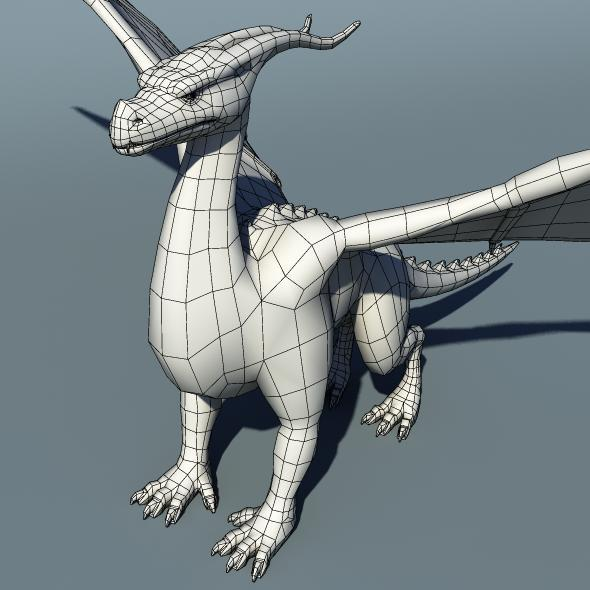
\includegraphics[width=2.5in]{dragon}
\caption{A mesh graph where lines correspond to edges and intersections of lines correspond to vertices.}
\label{fig_mesh}
\end{figure}

\begin{figure*}[ht]
\centering
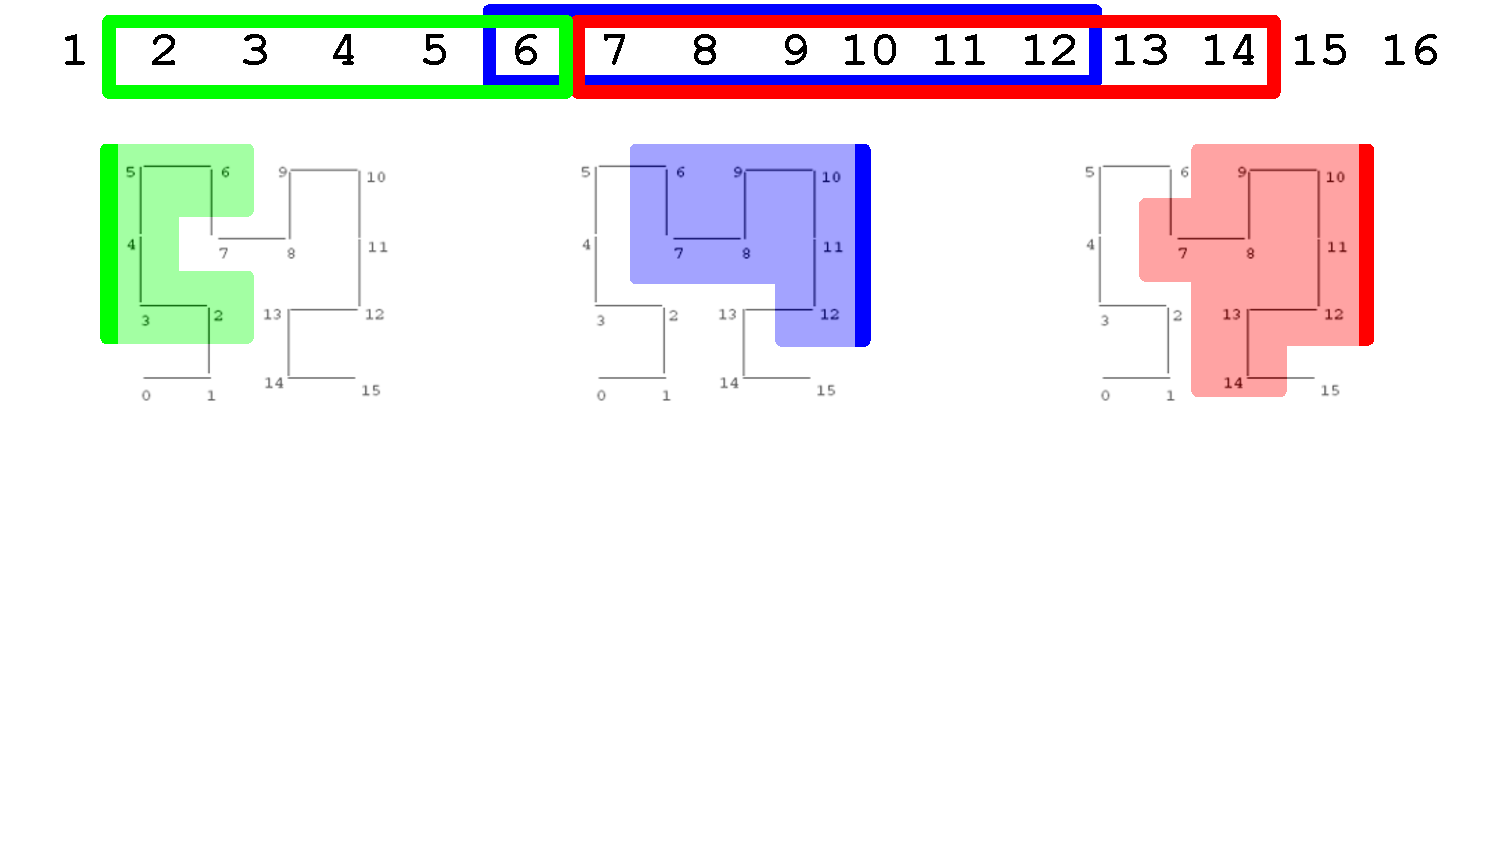
\includegraphics[trim=0cm 7cm 0cm 0cm, width=\textwidth,keepaspectratio]{hilbert_compact}
\caption{We see here that compact sets of vertices (represented by the green, red, and blue regions) in 2D space generally map to contiguous sets of Hilbert indices (indices are indicated on the Hilbert curve). The same holds in 3D space. So by ordering the vertices of a mesh graph by Hilbert index, connected vertices, which tend to be nearby in 3D space, are also nearby in the vertex array.}
\label{fig_hil_comp}
\end{figure*}

\begin{figure}[!t]
\centering
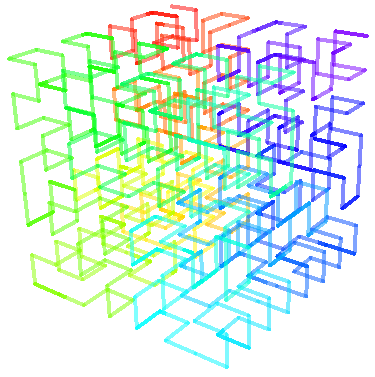
\includegraphics[width=2.5in]{hilbert3d}
\caption{A Hilbert curve tracing out the 3D space bounded by the box.}
\label{fig_hil3d}
\end{figure}

In this work, we optimize a graph processing framework for a specific workload: physical mesh simulations. A mesh graph is embeddable in 3D space, and an example is shown in Figure \ref{fig_mesh}. Mesh graphs have the nice property that we can partition them into sets corresponding to arbitrary contiguous regions in physical space, and edges cross out of a particular set only from vertices near the boundaries of its physical region. Thus, the number of edges crossing out of a set is proportional to the surface area of its physical region, which is a fairly small quantity relative to the number of vertices, especially when the region has large volume.

Taking advantage of these properties, we use a novel method based on space-filling curves to split up an input mesh graph across machines to limit inter-machine communication. We then optimize performance on individual machines by evaluating a number of techniques for the scheduling of vertex updates that hit different points in the cache/TLB locality and parallelism design space. Some of our results yield insights for more general classes of graphs.

% Discussion of BSP vs. Gauss-Siedel?

\section{Dealing with Distributed Execution}
Since an update function can only be run on a vertex if its neighbors are at most one iteration behind, we need to incur network traffic on every iteration to communicate vertex values for edges that cross machines. This can be done in a few ways. First, when an update function is being run on a vertex, it can fetch the values for neighbors on different machines and then run the necessary computation. This synchronous approach seems less than ideal, since the network traffic falls on the critical path of the iteration -- it is very likely that vertices that are capable of being updated without any network requests are waiting idle as the network requests complete.

Thus, an asynchronous approach is generally preferable. Our approach is as follows. For each edge that crosses machines, we declare one endpoint vertex as the predecessor and the other as the successor. Once the predecessor is updated, it sends its value to the machine to which the successor is assigned. Once the successor has received values from all of its predecessors, it can be scheduled for execution. If our partitioning of vertices across machines is good and there are many vertices on each machine that have no dependencies on external vertices and therefore can be scheduled at any time, then there will be minimal waiting for network messages. Our scheme ensures that we satisfy the constraint that vertex updates must appear to be processed in some global order -- in other words, both of the endpoints of an edge cannot be updated in some iteration based on the other's data from the previous iteration.

\begin{figure}[!t]
\centering
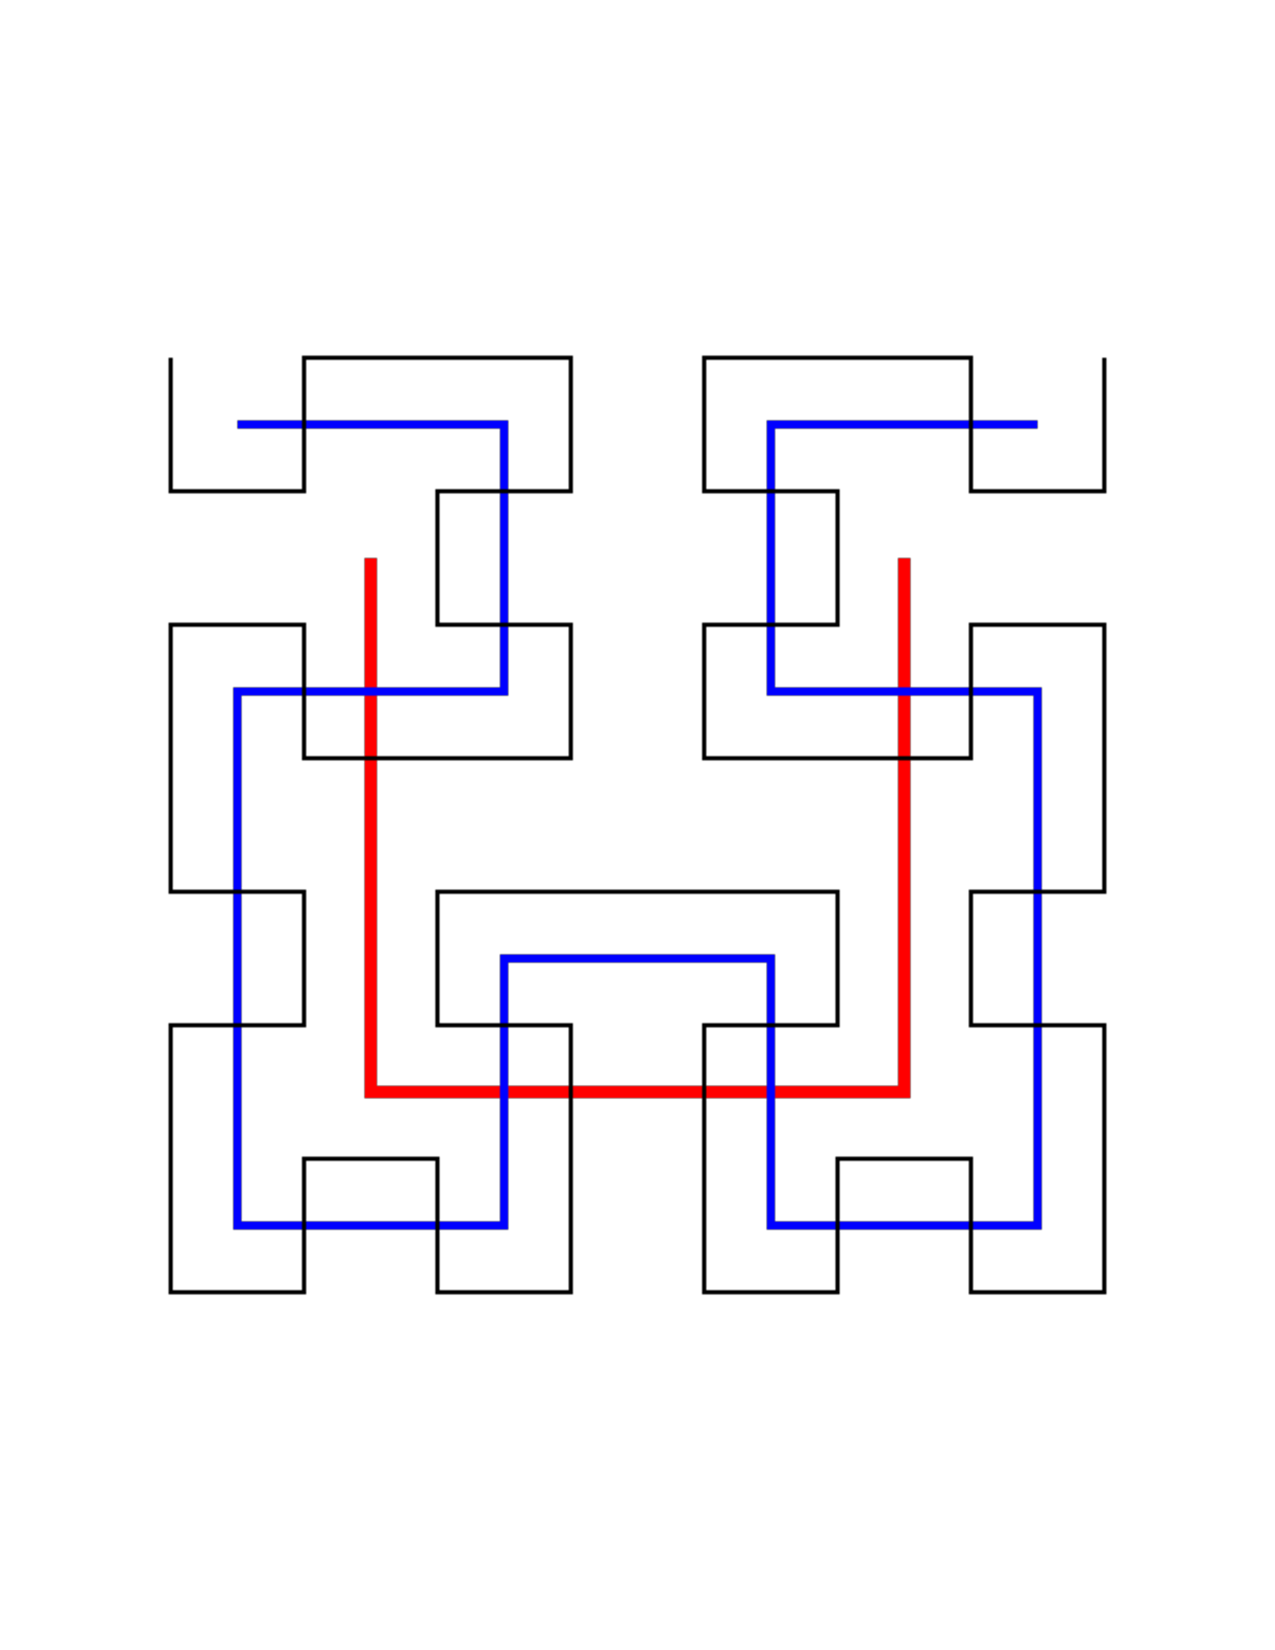
\includegraphics[trim=0cm 5cm 0cm 5cm, width=2.5in]{2d_hilbert}
\caption{The recursive process by which a 2D Hilbert curve is generated. This process can be generalized to 3D. The red curve is the first recursion level, the blue the second, and the black the third. Each edge of a Hilbert 'U' is turned into a 'U' in the next recursion level, and the space becomes more densely filled as we recurse. Notice that if we trace the black curve from its top left endpoint to its top right endpoint and assume that the Hilbert index is increasing as we trace, and if we map points in space to their nearest points on the Hilbert curve to assign them Hilbert indices, then nearby points are likely to have close Hilbert indices, as illustrated further in Figure \ref{fig_hil_comp}.}
\label{fig_hil2d}
\end{figure}

We partition vertices across machines using a technique based on space-filling curves. A 3D space-filling curve maps the real numbers to points in 3D space so that for an arbitrary point $p$ as we trace out more and more of the curve the distance from $p$ to the nearest point on the curve becomes smaller and smaller. We use a Hilbert curve, which has the property that if two points on the curve are relatively close together, then the real numbers that generated those points tend to be relatively close. A Hilbert curve in 3D space is shown in Figure \ref{fig_hil3d}.

Each vertex in a mesh graph can be assigned a particular coordinate in 3D space. Thus, we can draw a bounding box in 3D space around a mesh graph. We trace out a Hilbert curve over a finite portion of its domain mapping to points in the bounding box. We then assign each vertex in the mesh to its nearest point in the traced curve and mark the vertex with the real number that generated this point, which we will call the Hilbert index. We then sort the vertices by Hilbert index. Nearby vertices in the sorted order should be nearby in the physical graph. We can then split this sorted list into contiguous chunks, one for each machine in our cluster. Since each chunk should correspond to some contiguous region in 3D space, the number of edges crossing machines should be fairly small, as explained in the previous section. Figure \ref{fig_hil2d} gives more detail on how Hilbert curves are generated, and Figure \ref{fig_hil_comp} provides further intuition on why ordering by Hilbert index is effective.

\section{Fast Execution on Individual Machines}

Once we have a good vertex partitioning and a strategy for distributed execution, throughput depends largely on single-machine performance. We explore a number of schemes to this end.

\begin{figure*}[ht]
\centering
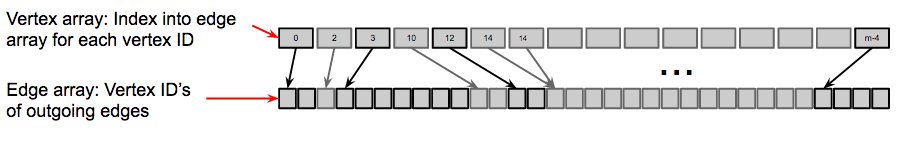
\includegraphics[width=\textwidth,keepaspectratio]{layout}
\caption{Organization of graphs in memory on a single machine.}
\label{fig_layout}
\end{figure*}

\subsection{Graph Representation in Memory}
We represent graphs in memory on a single machine as follows. We have an array of vertices and an array of edges. Each vertex contains data and a pointer into the edge array indicating the start of its list of edges. Adjacent vertices have adjacent edge lists. Each edge is simply a pointer into the vertex array. This organization is shown in Figure \ref{fig_layout}.

\subsection{Scheduling for Parallel Execution}
There are two major types of data-graph computations. The first is bulk synchronous parallel (BSP) and the second is Gauss-Siedel (GS). Certain simulation algorithms are designed for the BSP execution and others for GS, so we must consider both.

In BSP, otherwise known as double-buffering, in each iteration vertices are updated based on the values of their neighbors from the previous iteration. So any number of vertex updates can be performed in parallel, since for each vertex update we are reading from the buffers from the previous iteration and writing to a different buffer for the current iteration, so there are no races. Thus, it is easy to achieve high parallelism -- we can simply perform updates in a parallel loop over the list of vertices.

In GS, there is a fixed ordering on the vertices, and the updates of the vertices appear to occur in this order. So the update of vertex $k$ uses the values of any neighbors with indices smaller than $k$ from the current iteration and the values of neighbors with larger indices from the previous iteration. Here, since each vertex has only one buffer for its state, achieving high parallelism is more difficult. In particular, we cannot update two neighboring vertices in parallel, because read set of one intersects the write set of the other, so the semblance of an ordering between the updates of the two vertices would disappear.

\begin{figure}[!t]
\centering
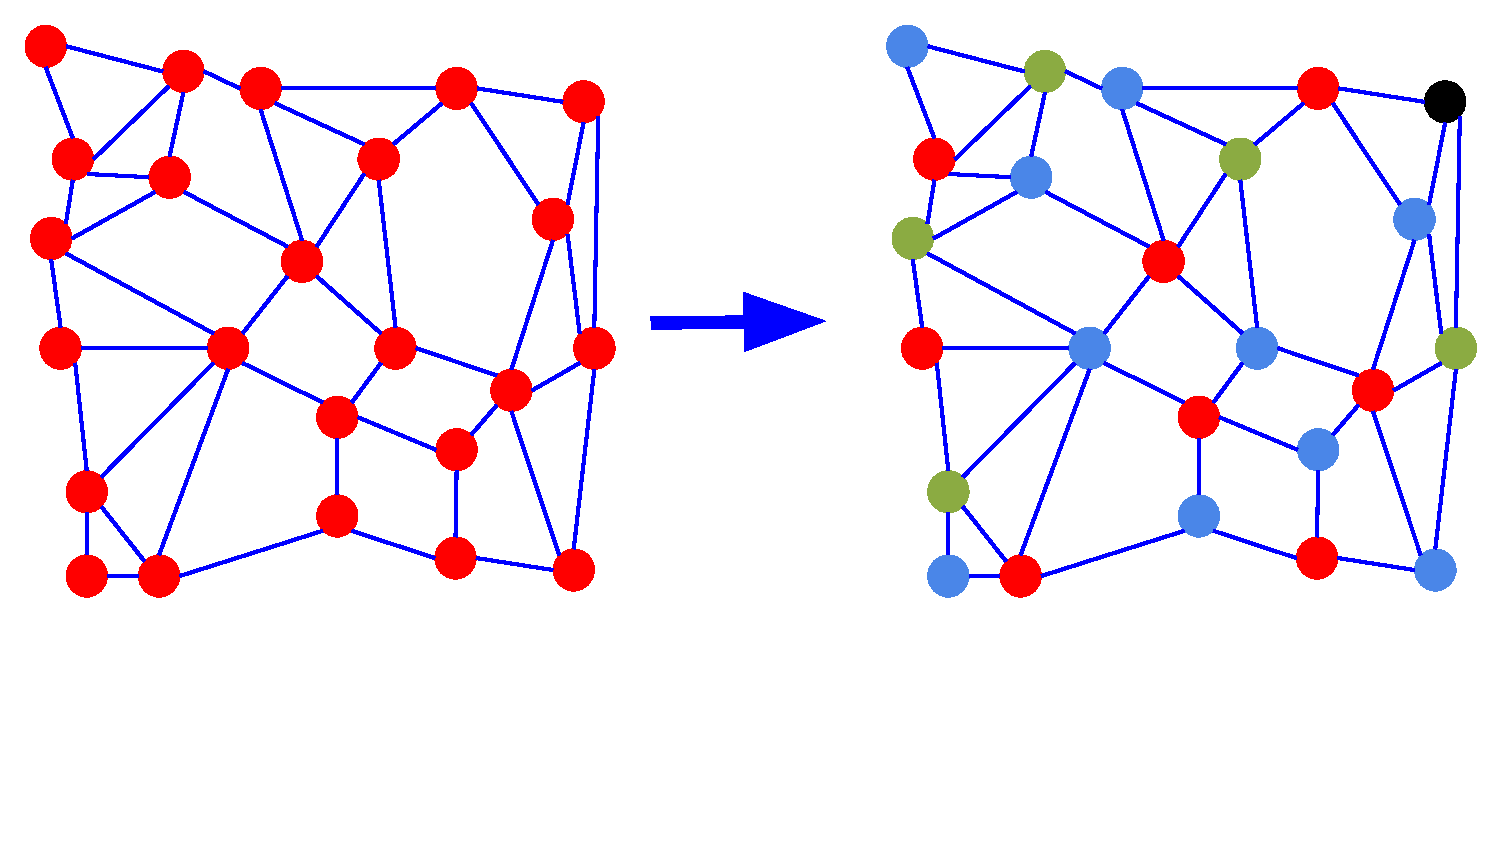
\includegraphics[width=2.5in]{chromatic_scheduling}
\caption{A graph colored so that no two neighbors have the same color and so that all vertices of a single color can be updated in parallel.}
\label{fig_chrom}
\end{figure}

There are two major approaches for parallel scheduling in the GS case. The first is coloring \cite{chromatic}. If we color a graph so that no two neighboring vertices have the same color, we can safely execute the updates for vertices of the same color in fully in parallel. The reason is that if any vertex's data is being written by some thread, it cannot be read in parallel by another thread because this would require a neighbor of this vertex to be updating concurrently, which is impossible. With the coloring strategy, we sort the vertex array (and the corresponding edge lists) by color and step sequentially through the colors, updating the vertices of each color in a parallel loop. An example graph that has been colored as described in shown in Figure \ref{fig_chrom}. 

\begin{figure}[!t]
\centering
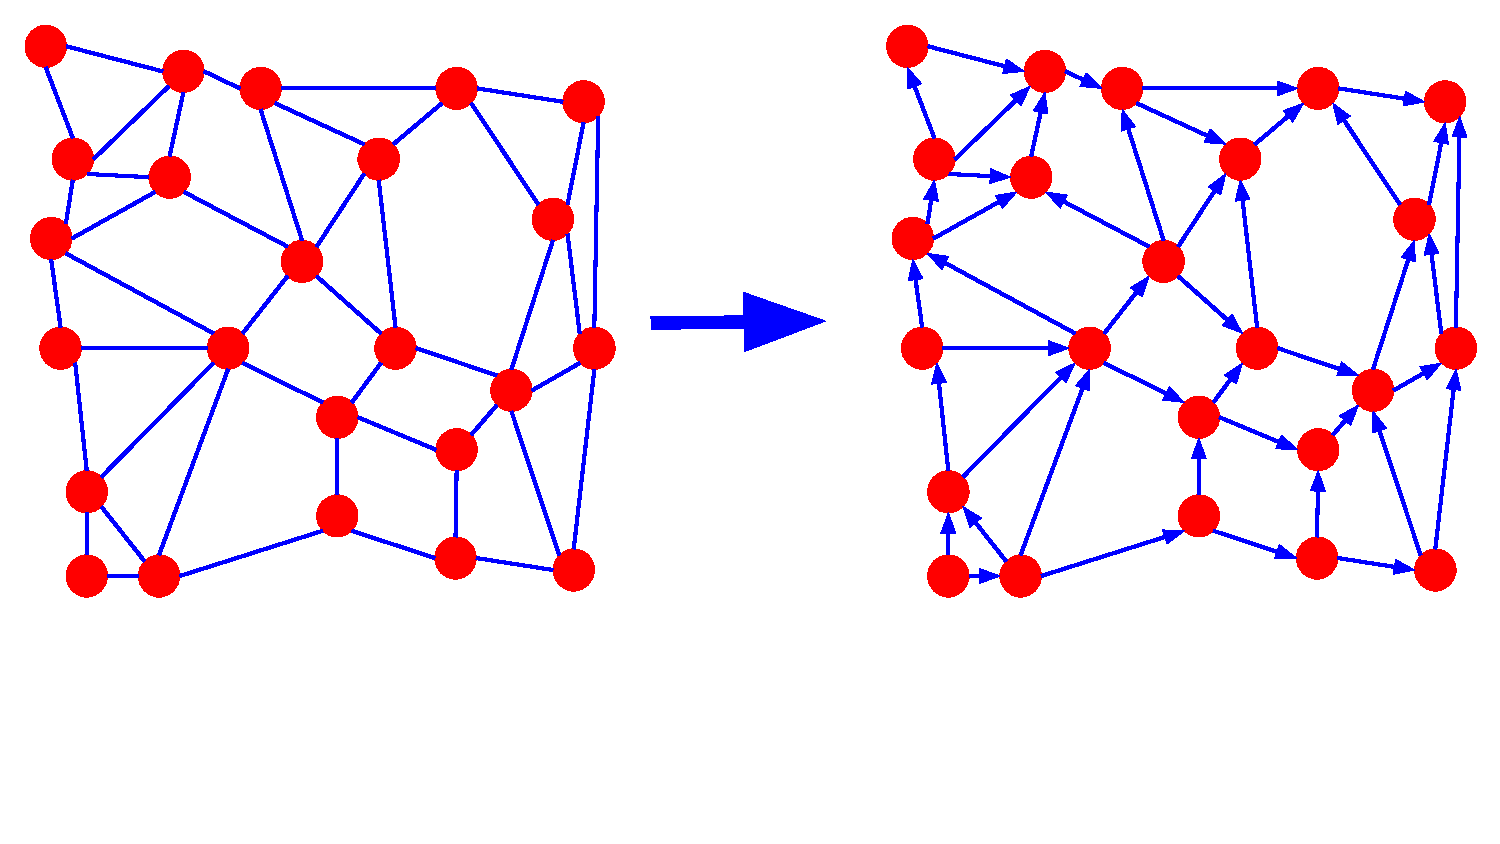
\includegraphics[width=2.5in]{dag_scheduling}
\caption{A graph whose vertices have been assigned priorities, resulting in the priority scheduling DAG shown at the right.}
\label{fig_dag}
\end{figure}

The other strategy is priority DAG scheduling \cite{dag}. This involves assigning each vertex a distinct priority, so that we can form a DAG from our graph by adding a direction to each edge such that the source is the endpoint vertex with higher priority. We assign each vertex a counter equal to the number of predecessors it has. We can start by executing all vertices with no predecessors (roots) in parallel. Once a vertex is complete, we atomically decrement the counter of each of its successors. If a vertex's counter becomes zero, we can spawn the update of this vertex as another parallel strand of execution. We thus attain fairly high parallelism at the cost of using atomics, which can involve expensive memory barriers on modern hardware. Once again, there can be no data races because two neighboring vertices cannot execute concurrently since one must be the predecessor of the other. Figure \ref{fig_dag} shows an example graph that has been made directed for priority scheduling.

Coloring-based scheduling performs very well when the graph can be colored with very few colors, since it essentially turns into the parallel BSP case. If many colors are required, priority DAG scheduling may become competitive. For our application of computations over mesh graphs, it is not a priori obvious which approach is better, so we consider both.

\subsection{Achieving Cache Locality}
If we update the vertices in the vertex array sequentially, as we do with coloring-based and parallel BSP scheduling, we get good cache locality (cache lines are processed completely after being fetched) on our accesses to the vertices being updated and to their corresponding entries in the edge array, which is also processed sequentially. Cache locality here includes data cache and TLB locality, since pages in the vertex and edge arrays corresponding to vertices being updated are processed completely after their first access. TLB misses have been shown \cite{tlb} to be a significant factor in the runtimes of data-intensive computations and are an important consideration for us.

While we get good locality on edge and vertex array accesses for vertices being updated, we get poor locality for accesses to the vertex array to fetch these vertices' neighbors. These accesses are essentially random unless we have sorted the vertex array in some locality-improving manner. Ideally we could store vertices' neighbors close to them in the vertex array. This would confer two benefits. First, TLB misses would fall since neighbors of a vertex will in most cases be stored in the same page as the vertex. Secondly, if a vertex being updated pulled neighbors that were yet to be updated into cache, those neighbors would be updated before they left cache, reducing cache misses.

These considerations suggest that ordering vertices in the vertex array by breadth-first search (BFS) level (using an arbitrary vertex as the source for the BFS) would be helpful. A vertex at BFS level $n$ can only have neighbors at BFS levels $n-1$ and $n+1$; if there was a neighbor at a smaller level, the vertex would have smaller level than $n$, and there can be no neighbors at levels greater than $n+1$ if the vertex is at $n$. Thus, if BFS levels are fairly small, ordering the vertices by BFS level would result in nearby neighbor accesses as desired. BFS levels are generally bounded in size in mesh graphs; they grow at first, but once the largest cross-section of the mesh is reached, successive levels should have similar size.

Another simple scheme is to order vertices by Hilbert index. As described in Figure \ref{fig_hil_comp}, adjacent vertices in mesh graphs are nearby in 3D space and therefore will have close Hilbert indices.

In the parallel BSP case, these orderings work perfectly, since we can always perform updates in a parallel loop over the vertex array, regardless of the ordering of vertices. 

In the parallel GS-coloring case, the problem with ordering the entire vertex array by BFS level or Hilbert index is that there are no longer defined sequential regions that we can assign a single color and over which parallel update loops can be run -- since any two adjacent vertices could be neighbors -- so parallelism is lost. Normally, when doing coloring-based scheduling, we order the vertex array by color, but there is no ordering specified within each color, so we can try order the vertices of each color in a cache-efficient manner, say by BFS level or Hilbert index. The problem with this is that the neighbors of a vertex are guaranteed to be of different colors than the vertex itself, so accesses of neighbors will certainly miss in cache. Thus, there is not much to be gained by ordering within each color, since locality of access to the neighbors of vertices being updated is what we really desire. In short, color-based scheduling seems to be cache-unfriendly. Indeed, our results show conclusively that for mesh graphs, color-based scheduling is trumped by priority DAG scheduling -- whose excellent cache behavior outweighs added overheads from atomics -- in the GS case.

In the case of priority DAG scheduling, cache behavior is very different from the parallel BSP or parallel GS-coloring cases. We lose some of the locality of access to the vertex and edge arrays for vertices being updated that we have in the sequential processing case. This is because for every vertex we update we do not necessarily update other vertices on the same cache line at around the same time. Of course, this is only relevant if there are several vertices stored on every cache line, which depends on the size of each vertex. But we are not without victories: when we update the last predecessor of some node we immediately afterwards update that node, at which point is hot in cache. So accesses to neighbors of vertices being updated do not have worst-case cache behavior as they do in the coloring case.

\begin{figure}[!t]
\centering
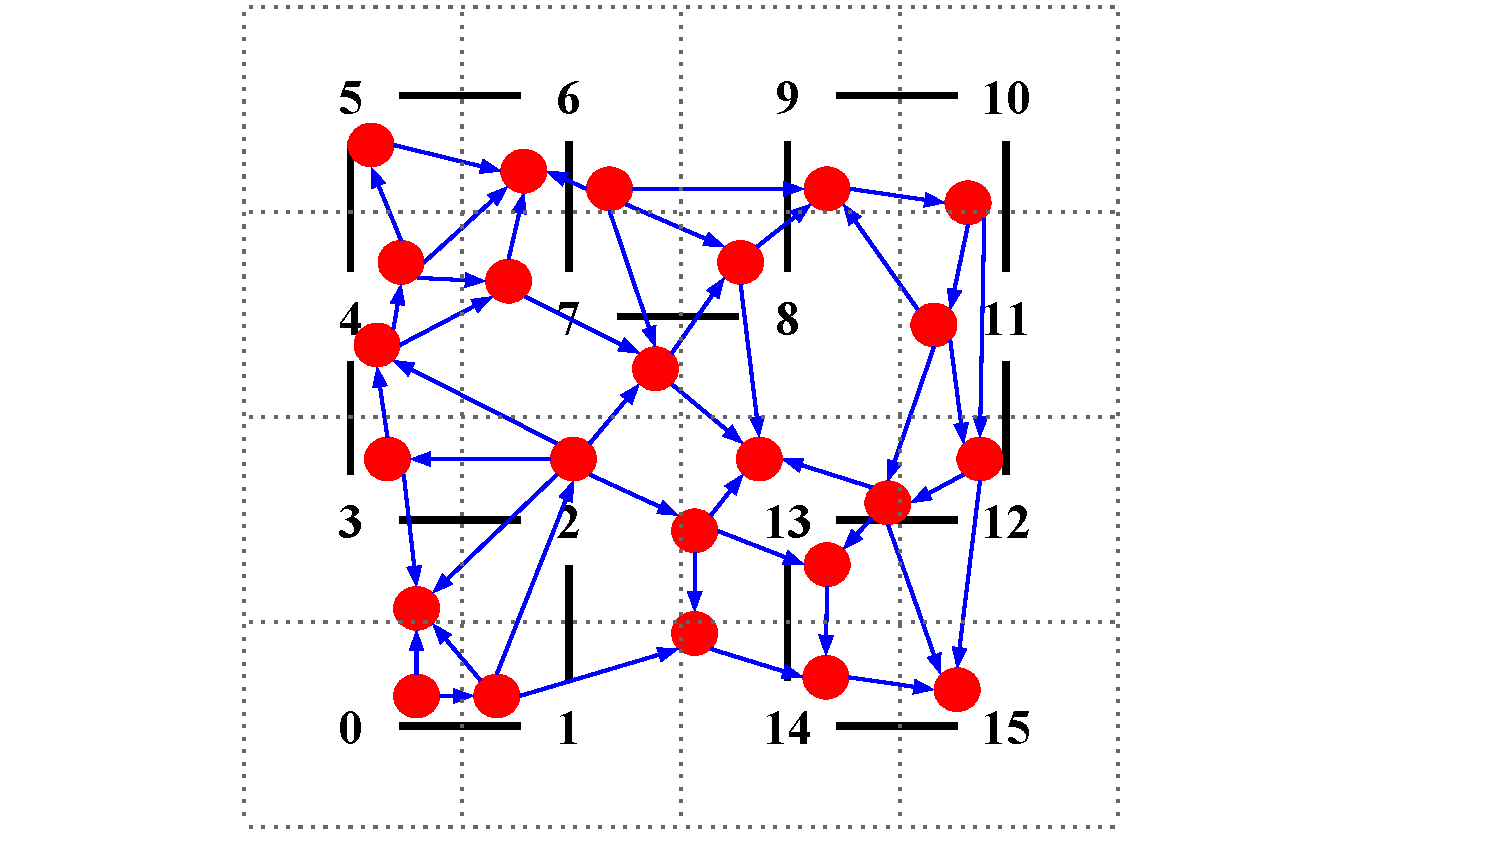
\includegraphics[trim=6cm 0cm 8cm 0cm, width=2.5in]{hilbert_priority_function}
\caption{A mesh whose vertices have been mapped to their nearest corners on a 2D Hilbert curve. Each corner on the Hilbert curve has an index, which becomes the priority of any associated vertices. A priority DAG is induced over the graph as shown. Note that here edges are drawn from low priority vertex to high priority vertex, which is the opposite of the convention used in the text. Edges between vertices with equal Hilbert index have arbitrary direction. Observe that in general vertices are connected to other vertices of nearby Hilbert index, so if the vertex array is sorted by Hilbert index, then neighbor accesses will exhibit good locality. There are also many chains of increasing priority, so neighbors that have been accessed for an update will tend to soon be updated themselves, which is also good for cache efficiency.}
\label{fig_hil_prio}
\end{figure}

\begin{figure}[!t]
\centering
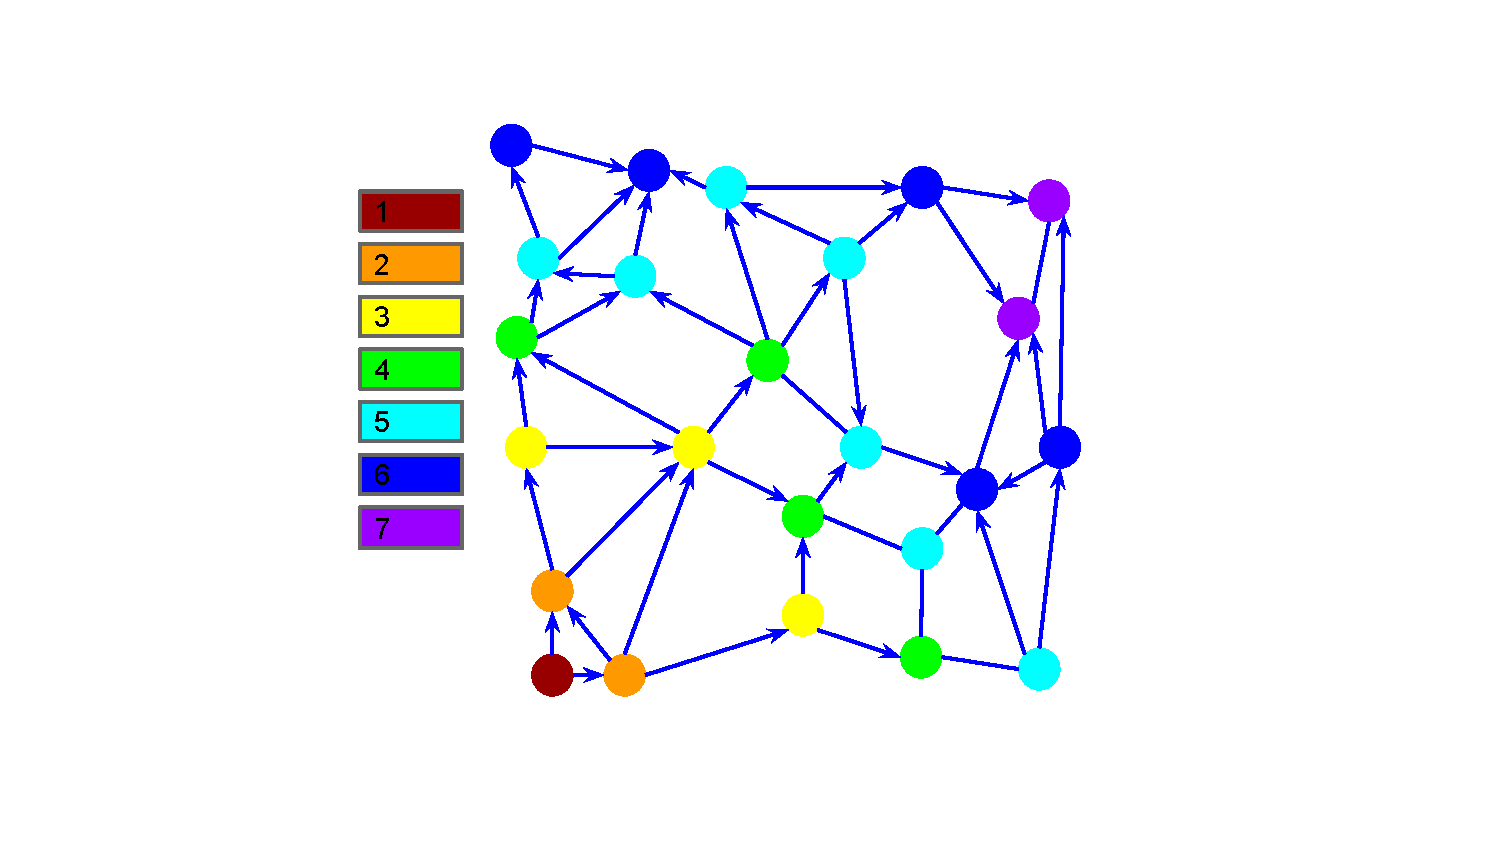
\includegraphics[trim=8cm 2cm 8cm 2cm, width=2.5in]{bfs_priority}
\caption{A mesh (the same as in Figure \ref{fig_hil_prio}) whose vertices have been assigned priorities equal to their BFS level, with the red vertex in the bottom left corner being the source of the BFS. The legend on the left shows the color given to vertices of each level. A priority DAG is induced over the graph as shown. Note that here edges are drawn from low priority vertex to high priority vertex, which is the opposite of the convention used in the text. Edges between vertices with equal BFS level have arbitrary direction. Observe that vertices are connected to other vertices of nearby BFS level (within $\pm 1$), so if the vertex array is sorted by BFS level, then neighbor accesses will exhibit good locality assuming that BFS levels are small. There are also many chains of increasing priority, so neighbors that have been accessed for an update will tend to soon be updated themselves, which is also good for cache efficiency.}
\label{fig_bfs_prio}
\end{figure}

For ideal cache behavior, the story is similar to the sequential processing case. We would like for neighborhoods of nearby vertices to be stored fairly contiguously in the vertex array so that accesses to neighbors of vertices being updated tend not to cause TLB misses. We would also like these neighborhoods to be updated completely in some small time window so that fetched neighbors are updated before they leave cache. Achieving the first objective is possible by using a BFS- or Hilbert-based ordering as described above. Achieving the second objective is much harder with DAG scheduling because the order in which vertices are updated is unclear. However, if we assign each vertex a priority equal to its BFS level or Hilbert index, there should be long chains of nearby vertices with monotonically decreasing priority that will be processed sequentially with high cache locality. (Of course, not all chains with monotonically decreasing priority can be processed continuously since some vertices may have unsatisfied dependencies, but it should be possible for some.) In the BFS case this is because there is high likelihood that there will be chains of vertices with decreasing BFS level since BFS level tends to move in one direction as we traverse from neighbor to neighbor. Similarly, in the Hilbert case, Hilbert index also tends to rise or fall continuously through a compact physical region, where there will be many connected vertices. Figures \ref{fig_hil_prio} and \ref{fig_bfs_prio} explore Hilbert index- and BFS level-based priority DAG scheduling on a 2D mesh.

%Draw parallel to cache-oblivious?

\subsection{Considering Parallelism}
% atomics, barriers in the priority DAG case
% cache transfers across processors are fast -- so as long as the data is in some cache, we are OK (not for TLB though) ... BUT
% Cilk -- steals high in the tree
We have been considering parallel scheduling algorithms in our prior discussions, but it is important to explicitly examine how parallelism improves performance and how it can potentially trade off with cache efficiency.

We discussed cache behavior above with the implicit assumption that cache behavior in a multiprocessor execution is very similar to its counterpart in a uniprocessor execution. This turns out to be generally true when using the Cilk runtime system \cite{cilk} for parallelization, which we do in this work. We consider specifically the cases of BSP execution and GS-priority DAG.

In BSP execution, we use a parallel Cilk loop over our vertex array to perform updates. Parallel loops are implemented in Cilk with recursive divide-and-conquer over the loop index range, with each piece of the index range being recursively spawned as a logically parallel strand of execution. Spawned strands of execution in Cilk run on the same processor core as the strands that spawned them, unless another processor core has run out of work and needs to steal. Steals, though, occur at the highest possible level of the spawn tree of the processor being stolen from. Thus, only very large spawned pieces of the index range will be stolen, and large contiguous stretches of the index range will therefore be updated on a single core, achieving the cache locality described above for parallel BSP.

In GS-priority DAG, the analysis is even simpler. If there are chains of vertices with decreasing priority that can be processed continuously as described above (due to BFS- or Hilbert- based priority assignment), then they will be processed on a single core unless a steal of some of the work occurs. But it has been shown \cite{cilk} that if a program has sufficient parallelism, steals are infrequent. So in general when we have such vertex chains we will see single-core cache behavior, which is exactly what we want.

\begin{figure*}[ht]
\centering
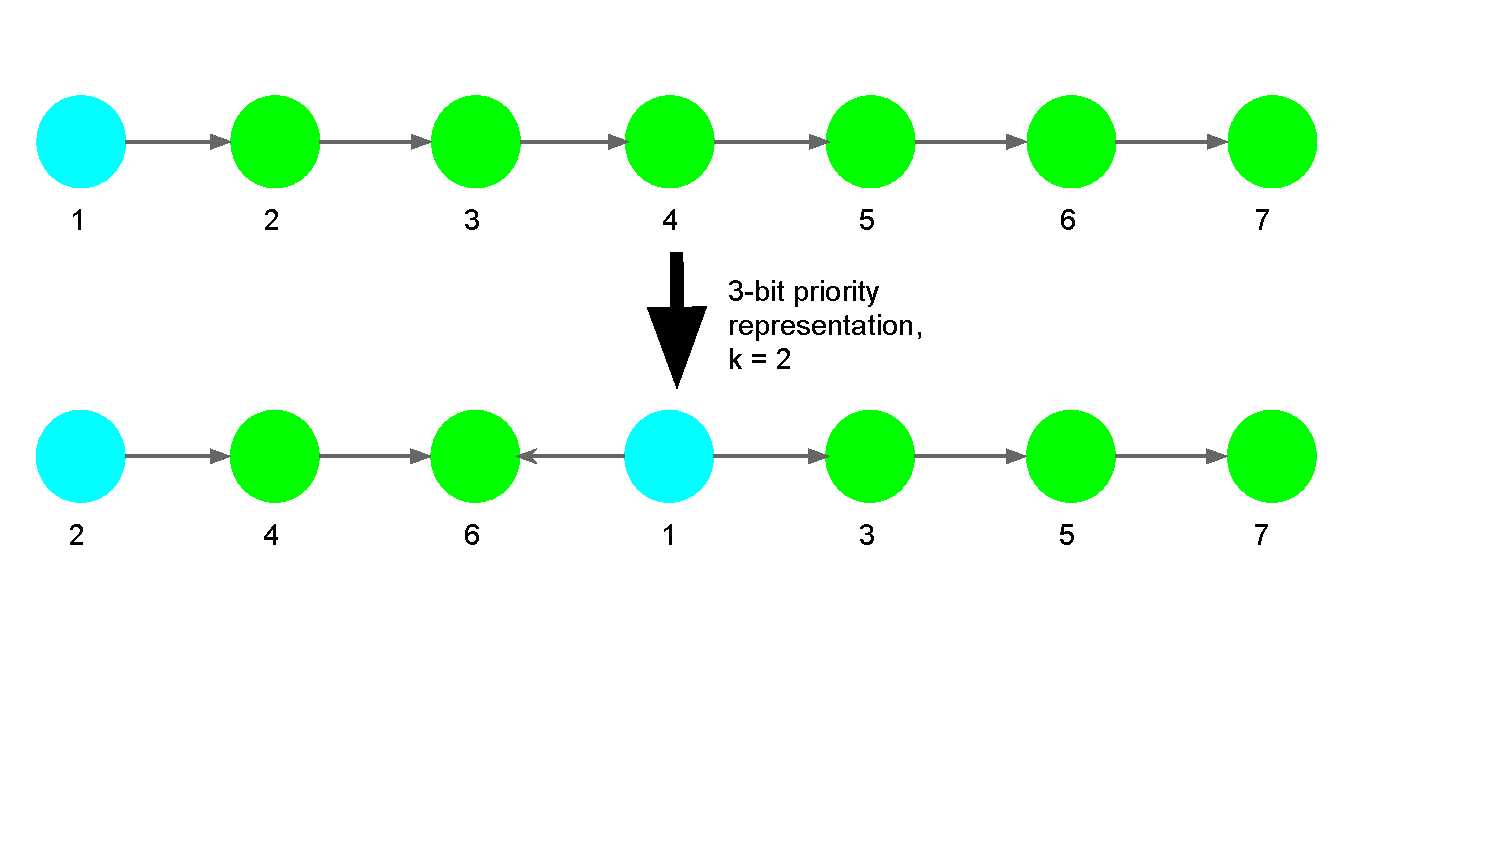
\includegraphics[trim=0cm 5cm 3cm 2cm, width=\textwidth,keepaspectratio]{k_effect}
\caption{An illustration of the effect of the parameter $k$, the number of lower-order bits from a node's priority that are made higher-order bits to break long chains of decreasing priority in order to increase parallelism. (Here again edges are drawn from low priority to high priority vertices, contrary to the convention in the text.) Priorities are listed under vertices. In the original graph at the top, there is no parallelism since updates must proceed from left to right, one after another. After reprioritization with $k = 2$, there are now two roots with no dependencies (colored light blue), so their updates (and those of their successors) can be performed in parallel.}
\label{fig_k}
\end{figure*}

% priority bits discussion, another figure for this? and another figure for BFS
It is important to note that long decreasing-priority vertex chains help cache efficiency but hurt parallelism, since they are a serial bottleneck. This is because vertices in such chains, by the laws of priority DAG scheduling, must execute one after another. Consider the case where the decreasing-priority chain includes all of the vertices in the graph. Then there is absolutely no parallelism because no two updates can execute in parallel. So we must strike a balance between having chains that are long enough, so that we have good cache efficiency, but not so long that parallelism is reduced to nothing. Our solution here is to not directly assign every vertex a priority equal to its BFS level or Hilbert index. Instead, we take the BFS level or Hilbert index, which we assume to have $n$ bits, and swap its bottom $k$ bits with its top $n-k$ bits. Thus, we limit the expected length of decreasing priority chains to around $2^k$, since after this number of vertices the upper $k$ bits of the priority should reset back to a high value. $k$ is a parameter that we tune to get parallelism just sufficient to saturate the cores on our evaluation machines, ensuring that cache efficiency remains high. Figure \ref{fig_k} illustrates the effect of setting $k$ on a simple example.

\section{Results}

\subsection{Evaluation Methodology}
We first wrote a script to generate mesh-like graphs. This script generated some number of vertices by sampling from a uniform distribution over a 3D space, and then connected each vertex to a random number of its nearest neighbors. We used Cilk to implement the parallel scheduling algorithms described above, using the graph layout described in Figure \ref{fig_layout}. We evaluated the algorithms on our generated mesh graphs on a 12-core, dual-socket Intel Xeon X5650 CPU with around 20 GB of available memory.

\subsection{Execution Times and Discussion}
We focus on single-machine optimization in our results and leave distributed implementation and performance analysis to future work. Runtimes and performance counter values for different scheduling approaches and vertex orders are shown in Figure \ref{fig_result}.

As expected, in both the BSP and priority DAG cases, Hilbert- and BFS-based ordering and priority assignment outperform the baseline. Interestingly, Hilbert appears far superior to BFS. In the BSP case, this is because BFS turns out not to achieve the key property of a cache-efficient vertex ordering: adjacent vertices are oftentimes far apart in the vertex ordering. The key reason for this is that in our generated graphs, BFS levels are often very large. On the graph we used to get the results in Figure \ref{fig_result}, the average BFS level had 44,642 vertices. Our goal was to make accesses to neighbors hit in both TLB and data cache. With levels of this size, accesses to neighbors, which will be in the same level as the current vertex or one of the adjacent levels, could be as far as around 80,000 vertices away from the current vertex and on average a few tens of thousands of vertices away. Assuming pages of around 4 KB in size and vertices of a few tens of bytes, the page translations for a few BFS levels can easily fit in TLB, so neighbor accesses are likely to hit in TLB, which is why we see that BFS TLB numbers are similar to their Hilbert counterparts. But the story is not the same for data caches, as the numbers indicate. By the time a neighbor that is pulled into cache during a vertex update is updated itself, which may be as many as 80,000 updates later, it is likely to have been evicted from cache. So data cache locality is where BFS really loses to Hilbert. Evidently, the Hilbert ordering is able to keep adjacent vertices in a much smaller neighborhood in the vertex array. Although we predicted that BFS levels would be fairly small in mesh graphs, and indeed they are smaller than they would be on random graphs, they turned out to be too large to be of much use from the perspective of cache efficiency.

In the priority DAG case, the relative performances of BFS and Hilbert are similar, for similar reasons. The main factors affecting priority DAG performance are nearness of neighboring vertices in the vertex array and the presence of sufficiently long chains of vertices with decreasing priority that do not have too many other dependencies outside a neighborhood of vertices a few edges away. BFS performs poorly on both of these fronts. Accesses to the neighbors of a vertex being updated may be in an adjacent page rather than the same page as the vertex being updated, and unlike in the BSP case, adjacent pages may not be in TLB. Regarding the second factor, under a BFS level-based prioritization scheme, a single vertex may be dependent on vertices from across the graph with lower BFS level, especially if the graph is well connected and vertices are generally reachable from most others. Thus, there are few chains of decreasing priority that can be executed in quick succession, since vertices generally have to wait on dependencies from across the graph, and this hurts temporal locality and cache efficiency. Hilbert-based prioritization is better at preventing multiple decreasing priority chains from converging and creating such dependencies, since in general disparate regions of the mesh correspond to disjoint portions of the Hilbert index space and there is no factor (like the explicit dependence of BFS level on vertex adjacency) that makes the formation of many decreasing priority chains passing through many nearby regions and terminating at a single region particularly likely. In effect, in the BFS setting, for a particular region and vertices in that region, every neighboring region will have some vertices of higher priority that can contribute to decreasing priority chains extending into the region. In the Hilbert setting, many neighboring regions will contain vertices only of lower priority, so long chains of decreasing priority coming from all directions becomes unlikely. But there will still be \textit{some} long chains of decreasing priority, and when they form they will tend not to have many other dependencies, which is good for cache efficiency.

It is interesting also to consider the optimal values of the parameter $k$ for the priority DAG case. In all serial executions, $k = 0$ was optimal, which makes sense because higher $k$ helps only in that exposes additional parallelism, at the expense of some cache efficiency. The fact that $k = 0$ was optimal for parallel BFS-based scheduling confirms that BFS prioritization did not result in long decreasing priority chains with few dependencies that needed to broken for additional parallelism. In contrast, $k = 18$ was optimal for the parallel Hilbert case, indicating that many such chains were present. It is clearly better if these long chains exist, because we can always split them up to get the necessary parallelism by appropriately setting $k$, and if they are not present we lose out in terms of cache efficiency.

It is also worth examining the differences in cache misses between corresponding serial and parallel executions. The parallel executions almost always have significantly more cache misses. This is because two chunks of work that in the serial case executed close together in time and shared data, resulting in good cache locality, may in the parallel case be executed on separate cores due to work stealing, eliminating the locality. The reason that the increase in cache misses from the BSP BFS serial to parallel execution is much higher than other in other serial-to-parallel transitions may be that as mentioned previously, neighbor references are more distant than in the Hilbert case, so it is more likely that the update for a neighbor of a vertex will execute on a different core (since steals in Cilk tend to happen high in the spawn tree).

Finally, we should return to the question of coloring-based GS execution. We noted earlier that coloring prevents us from ordering the vertices in a cache-efficient manner, so at best coloring could get the performance of the input (random) vertex order BSP execution (since we did not include the overhead of swapping BSP buffers at the end of each round in our measurements), since BSP involves a parallel loop over the entire vertex array while coloring must settle for sequentially executed parallel loops over smaller pieces of the array. But the data make clear that the random BSP case is slower than the Hilbert-based priority DAG case, so clearly for GS execution on mesh graphs priority DAG scheduling with a cache efficient vertex ordering and prioritization is superior to coloring.

\begin{figure*}[ht]
\centering
\resizebox{\textwidth}{!}{%
\begin{tabular}{ l c c c c c c }
Schedule \& Vertex Order & Serial Time (s) & Serial d-TLB Misses ($10^6$) & Serial d-cache Misses ($10^6$) & Parallel Time (s) &  Parallel d-TLB Misses ($10^6$) & Parallel d-cache Misses ($10^6$) \\
\hline
BSP \& Input & 4.01 & 450 & 656 & 1.26 & 451 & 680  \\
BSP \& BFS & 2.22 & 0.601 & 180 & 0.98 & 0.721 & 533  \\
BSP \& Hilbert & 1.24 & 0.482 & 80.9 & 0.33 & 0.566 & 123  \\
DAG \& Input & 9.92 & 447 & 590 & 1.76 & 420 & 614  \\
DAG \& BFS & 8.31 & 17.1 & 314 & 1.38 & 13.4 & 454   \\
DAG \& Hilbert & 5.52 & 0.553 & 123 & 1.02 & 0.788 & 162  \\
\end{tabular}
}
\caption{Execution times and performance counter values on a 10M-node mesh graph over three rounds of vertex updates for different execution schedules and vertex orderings. d-cache misses gives the number of data memory requests that could not be served by any level of cache. Serial code was obtained in each instance by simply eliding Cilk keywords. The input order is simply the order of the vertices in the input file passed to the program, which is essentially random from the perspective of cache efficiency. The optimal value of the parameter $k$ was 0 in all but the DAG \& Hilbert case, where it was 18.}
\label{fig_result}
\end{figure*}

% performance counters?
% BFS vertices per level (Vertices per level: 44642)
% k = 0 for all but Hilbert parallel, where it is 18
% cache misses way higher in BFS parallel case (generally increase in parallel because of steals and different core execution)
% why coloring is definitely worse

\section{Conclusion \& Future Work}
In summary, we have optimized the execution of algorithms that evolve 3D mesh graphs. Assuming that such algorithms can update each vertex in the mesh by considering only its neighbors, and taking advantage of the property that adjacent vertices in mesh graphs tend to be nearby in 3D space, we demonstrate that ordering and prioritizing vertices by the index of their nearest point on a Hilbert curve results in high cache locality when vertex updates are scheduled in both the sequential, bulk-synchronous parallel (BSP) and priority DAG styles. This is because vertices tend to be located on the same pages as their neighbors, so accesses to neighbors during updates often hit in TLB. Furthermore, vertices that are pulled into cache as part of the updates of their neighbors tend to be updated themselves before they are evicted from cache. We show speedups of up to 4 times over random vertex orderings. In memory-heavy (as opposed to computation-heavy) algorithms like those used for simulations on mesh graphs, cache efficiency can make a huge difference in performance.

We also show the interesting result that ordering vertices by BFS level does not produce nearly as large a performance improvement as Hilbert-based ordering. The problem is that BFS levels can be fairly large relative to cache sizes even in mesh graphs, so accesses to neighbors of a vertex, which are guaranteed to be in the same or immediately adjacent BFS levels, may not be particularly local in the vertex array. Furthermore, in the priority DAG case, there may be paths of decreasing BFS level (and therefore priority) from disparate parts of the graph to a different vertices in the same BFS level, so it may be hard to process entire BFS levels in a small window of time. It would be interesting to investigate what properties of mesh graphs tend to affect the size of BFS levels.

The other major area of future work is implementation and evaluation of distributed execution. As noted earlier in the paper, partitioning the graph across machines based on Hilbert index should result in minimal cross-machine communication, as the partitions on individual machines will correspond to contiguous regions of the mesh with outgoing edges only at the boundaries. So performance should scale nearly linearly with the addition of further machines, enabling us to tackle huge problem sizes.  
\ifCLASSOPTIONcaptionsoff
  \newpage
\fi

\begin{thebibliography}{1}
% more refs, Cilk ref at least
\bibitem{graphlab}
Y.~Low et. al. \emph{GraphLab: A New Framework for Parallel Machine Learning}. \textit{UAI}, 2010.

\bibitem{hadoop} 
\emph{Hadoop}. http://hadoop.apache.org. 2015.

\bibitem{dag}
W.~Hasenplaugh et. al. \emph{Ordering Heuristics for Parallel Graph Coloring}. \textit{SPAA}, 2014.

\bibitem{chromatic}
T.~Kaler et. al. \emph{Executing Dynamic Data-Graph Computations Deterministically Using Chromatic Scheduling}. \textit{SPAA}, 2014.

\bibitem{cilk}
M.~Frigo et. al. \emph{The implementation of the Cilk-5 multithreaded language}. \textit{PLDI}, 1998.

\bibitem{tlb}
K.~Goto et. al. \emph{On Reducing TLB Misses in Matrix Multiplication}. Working paper, 2002.

\end{thebibliography}

\end{document}


